\newpage
\chapter{Обучение на мрежата}
\label{chapter07}

Обучението при класическите многослойни изкуствени невронни мрежи е свързано с оптимизация на теглата, които характеризират връзките между отделните неврони. По своята същност задачата за обучение представлява числена оптимизация в многомерно пространство на реалните числа. През последните няколко десетилетия са разработени множество точни числени методи и множество евристични методи. В настоящата разработка акцентът пада над два метода (единият точен числен, а другият евристичен). Като точен числен метод софтуерната библиотека Encog предлага широко използваният метод с обратно разпространение на грешката (както и някои негови модификации). От групата на евристичните методи се използват генетични алгоритми с модификация на мутацията, според метода за еволюция на разликите. За реализацията на генетичния алгоритъм се използва софтуерната библиотека Genetic Algorithms - Apache Commons.

\section{Обратно разпространение на грешката}

При обратното разпространение на грешката, в работен режим, сигналите пътуват от входа на мрежата към нейния изход. Тренировъчните примери се прилагат в случайно определен ред, така че мрежата да не заучи схемата на подаване, а да развие своите обобщаващи способности. Общата допусната грешка се изчислява на изхода на мрежата и след това се връща по обратния път, от изход към вход, за да бъде изчислена грешката с която всеки неврон допринася. След определянето на индивидуалната грешка за всеки неврон се извършва числена корекция (според градиента) на теглата, които свърват невроните. Този обратен ход на пресмятане дава името на метода и също така го поставя в групата на точните числени методи, които разчитат на градиента за да извършат корекция в теглата. Същественото за обучението с обратно разпространение на грешката е, че активационната функция на неврона трябва да бъде диференцируема. 

\begin{figure}[h]
  \centering
  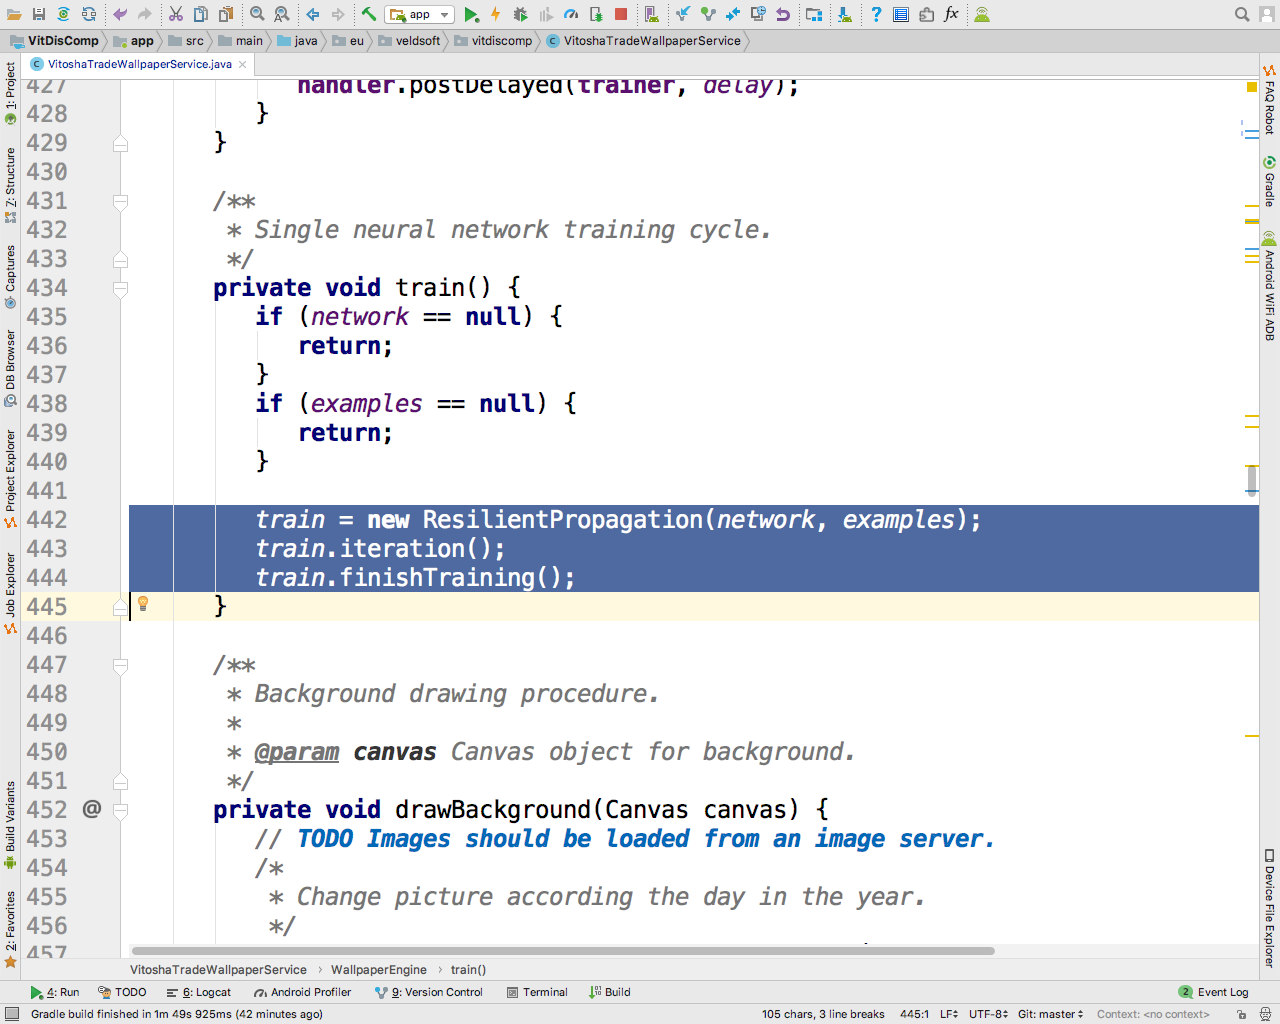
\includegraphics[height=0.45\pdfpageheight]{pic0173}
  \caption{Единична стъпка за обучение на мрежата.}
\label{fig:pic0173}
\end{figure}
\FloatBarrier

Библиотеката Encog позволява няколко възможности за обучение с точни числени методи и в настоящата разработка е избран метода Resilient Propagation, който представлява еластично обратно разпространение на грешката (Фиг. \ref{fig:pic0173}). Еластичното разпространение на грешката е модификация на основния метод в която модификация степента за научаване (learning rate) се определя динамично и не е само една стойност за цялата мрежа. При класическия подход с обратно разпространение на грешката степента за научаване е само една стойност, обикновено емпирично нагласена между 0.0 и 1.0. Най-често се използва 0.35, което е компромис между бързината за научаване и достигането на оптимална стойност за теглата (фината стъпка за нагласяне на телата в крайната фаза от обучението).

\begin{figure}[h]
  \centering
  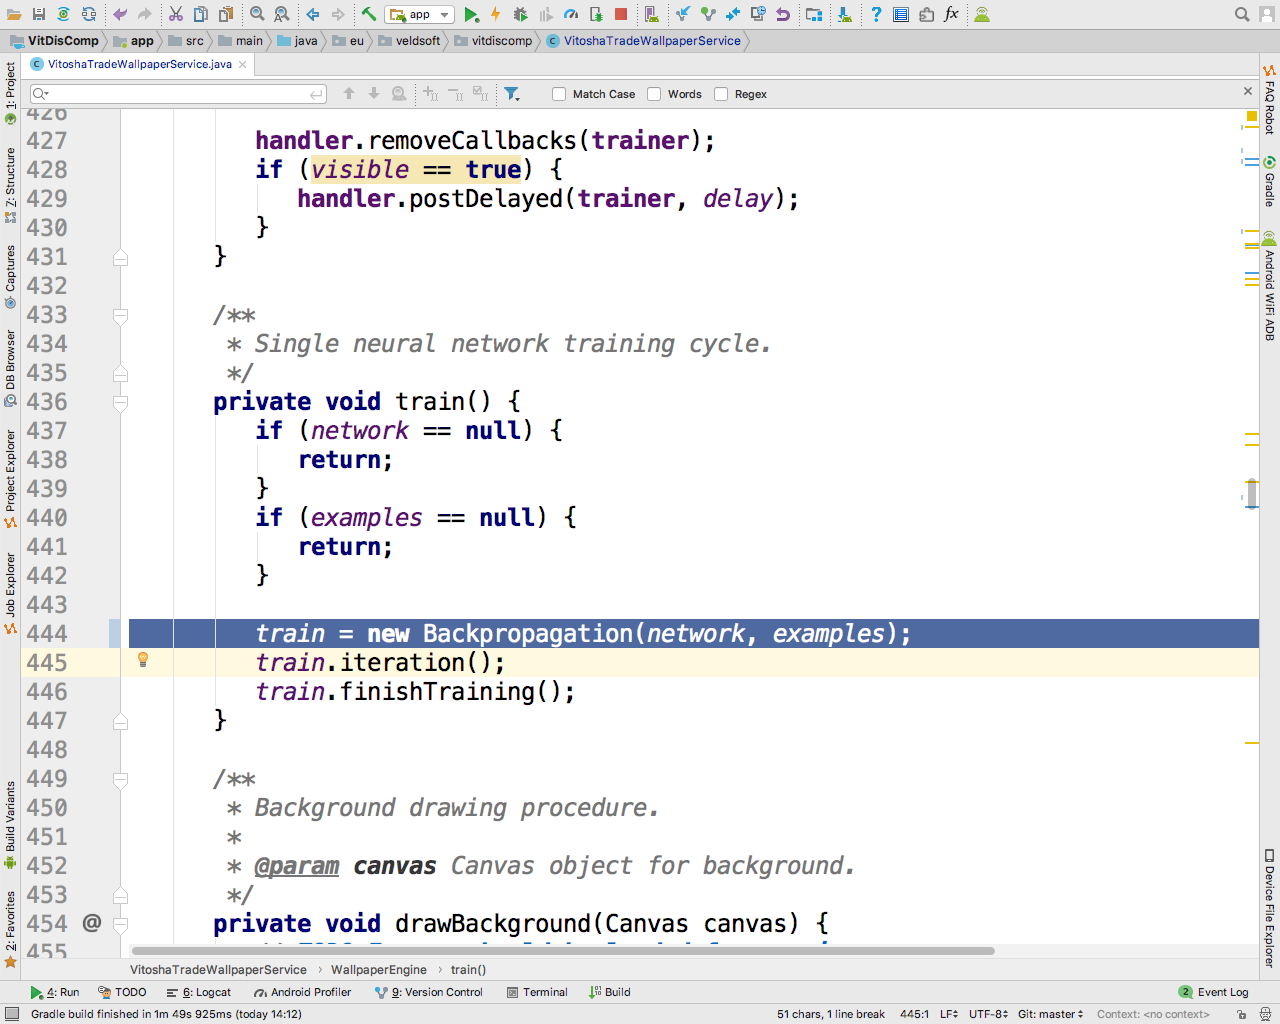
\includegraphics[height=0.45\pdfpageheight]{pic0174}
  \caption{Класическо обратно разпространение на грешката.}
\label{fig:pic0174}
\end{figure}
\FloatBarrier

Фактът, че библиотеката Encog е написана по каноните на обектно-ориентираното програмиране, позволява само с подмяната на един ред (Фиг. \ref{fig:pic0174}) от еластично обучение да преминем към класическо. 

\section{Генетични алгоритми}
